\documentclass{templateNote}
\usepackage{tcolorbox}
\usepackage{tabularx}
\usepackage{hyperref}
\usepackage{amsmath}
\usepackage{amssymb}
\usepackage{pdflscape}
\usepackage{tikz}
\usepackage{soul}
\usepackage{media9}
\usepackage{adjustbox}
\usepackage{pdfpages}
\usepackage{comment}
\usepackage{enumitem}
\usepackage{parskip}
% \usepackage[spanish,es-noquoting]{babel}

\begin{document}
\linklogoU{https://www.ubiobio.cl/w/}
\linklogoD{https://github.com/NicoGomezM}
\imagenlogoU{img/logo-ubb-txt-face.png}
\imagenlogoD{img/logoNGMFormal_sinF.png}
\titulo{Laboratorio 1: Intérprete de comandos en Linux}
\asignatura{Laboratorio Sistemas Operativos}
\autor{
    Nicolás \textsc{Gómez Morgado}
}

\portada
\margenes

% \section*{Ejercicios solicitados}

\textbf{Ejercicios:}
\begin{enumerate}
    \item Configuración inicial (mkdir, unzip). 2pts por ítem.
    \begin{enumerate}[label=\alph*)]
        \item Ubíquese en el siguiente directorio: /home/nombre\_de\_usuario, donde \\nombre\_de\_usuario es el nombre con el cual inició sesión.
        \item Cree una carpeta con nombre ssoo.
        \item Descargue el comprimido Lab1.zip, y descomprímalo dentro del directorio ssoo. Este será su directorio de trabajo. El directorio de trabajo será entonces: /home/nombre\_de\_usuario/ssoo/Lab1.
    \end{enumerate}
    \begin{center}
        \texttt{wget --no-check-certificate 'https://docs.google.com/uc?\\export=download\&id=1bVdayOoOvS2uykzWkwwKrxFpxT8fpDIP' -O Lab1.zip}
    \end{center}

    \begin{figure}[H]
        \centering
        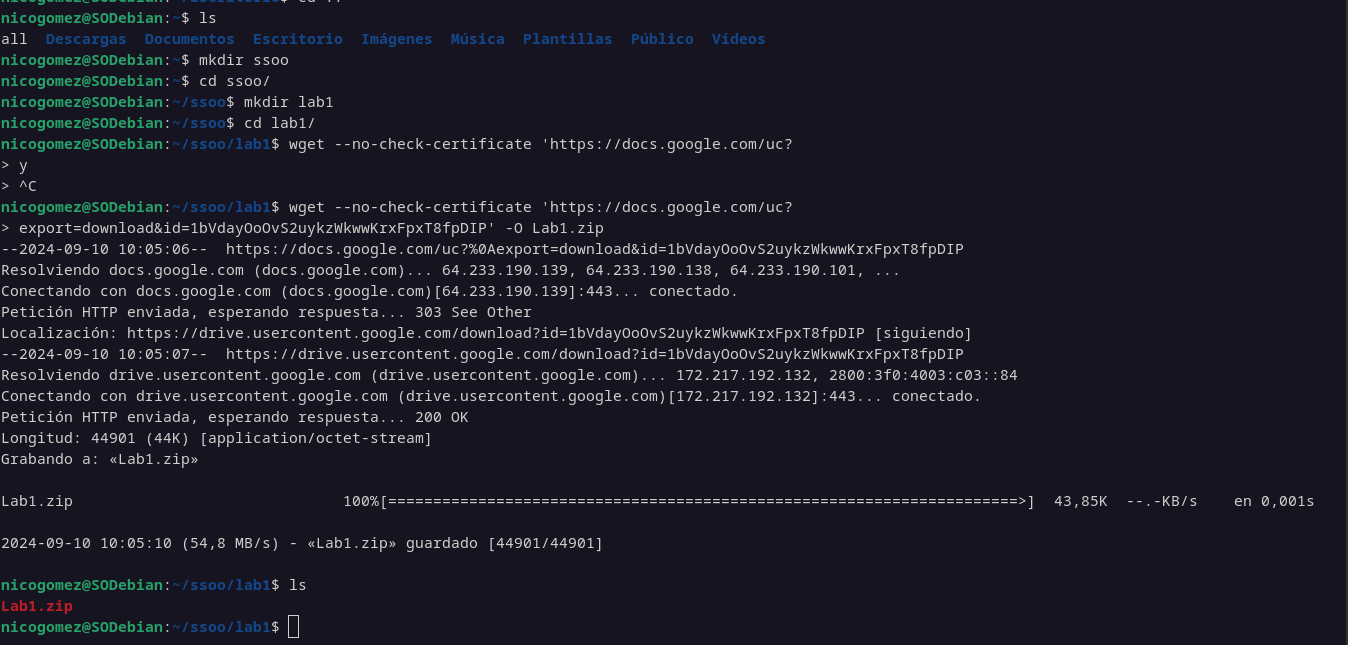
\includegraphics[width=\textwidth]{img/ejerc1.png}
    \end{figure}

    Para la realización de este laboratorio dispuse de una maquina virtual, por lo tanto el directorio de trabajo es \texttt{$\sim$/ssoo/Lab1} como se muestra en la figura anterior ya que trabaje desde el directorio raíz de la maquina virtual.
    Para la ubicación en el directorio utilize el comando \texttt{ls} para verificar que estaba en el directorio correcto, luego utilice el comando \texttt{mkdir ssoo} para crear la carpeta donde descargar el .zip, ingrese a la carpeta creada con \texttt{cd ssoo} y luego utilice el comando \texttt{wget} para descargar el archivo con el link proporcionado.
    \item Listando archivos (cd, pwd, ls). 2pts por ítem.
    \begin{enumerate}[label=\alph*)]
        \item Ubíquese dentro del directorio de trabajo y verifique que se encuentra ubicado en /home/nombre usuario/ssoo/Lab1
        \begin{figure}[H]
            \centering
            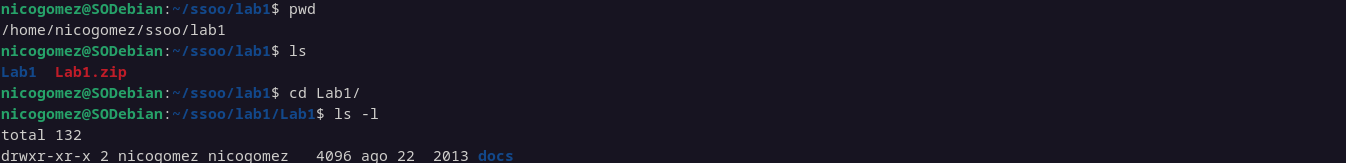
\includegraphics[width=\textwidth]{img/ejerc2a.png}
            Primero revise en que lugar estaba con \texttt{pwd} y luego liste los archivos (\texttt{ls}) para acceder a la carpeta descomprimida con \texttt{cd Lab1/}
        \end{figure}
        \item Despliegue la lista de archivos de manera simple. ¿Cuántos archivos y directorios hay?
        \begin{figure}[H]
            \centering
            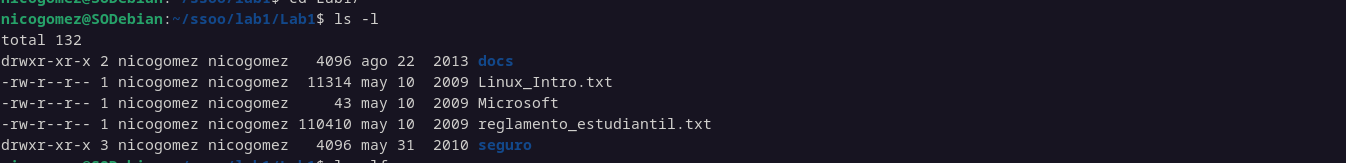
\includegraphics[width=\textwidth]{img/ejerc2b.png}
            Use el comando \texttt{ls -l} para ver los archivos en formato de lista y asi observar que existen 3 archivos y 2 carpetas (directorios).
        \end{figure}
        \item Ahora despliegue todos los archivos, incluso los ocultos ¿Cómo identifico archivos ocultos? ¿Cuál es el archivo oculto?
        \begin{figure}[H]
            \centering
            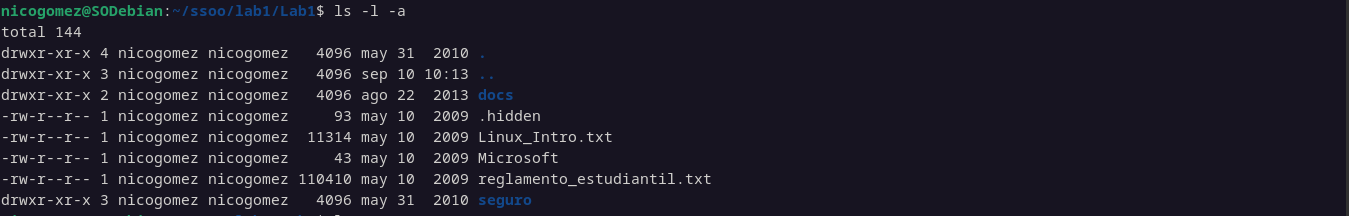
\includegraphics[width=\textwidth]{img/ejerc2c.png}
            Para esto use la combinación de comandos \texttt{ls -l -a} para ver los archivos ocultos (opción que otorga \texttt{ls -a}) y a su vez ver los archivos en formato de lista. Para este caso el archivo oculto es el nombrado \textit{.hidden} y se identifica por el punto al inicio del nombre.
        \end{figure}
        \item Liste primero los archivos más antiguos
        \begin{figure}[H]
            \centering
            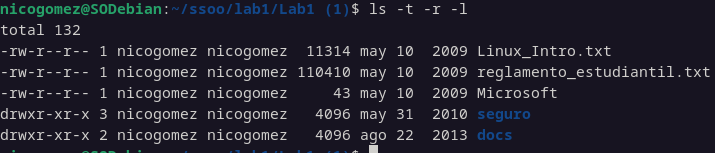
\includegraphics[width=\textwidth]{img/ejerc2d.png}
            Para este caso utilice el comando \texttt{ls -t -r -l} para listar los archivos por fecha, revertir el orden y listar respectivamente.
        \end{figure}
        \item Liste primero los archivos más pequeños
        \begin{figure}[H]
            \centering
            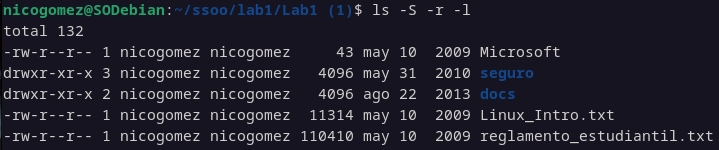
\includegraphics[width=\textwidth]{img/ejerc2e.png}
            Finalmente utilice para este caso la combinación \texttt{ls -S -r -l} para listar los archivos por tamaño, revertir el orden y listar respectivamente.
        \end{figure}
    \end{enumerate}
    \item Examinando el contenido de un archivo (cat, less, nano). 3pts por ítem.
    \begin{enumerate}[label=\alph*)]
        \item Despliegue el contenido completo del archivo Linux Intro.txt
        \begin{figure}[H]
            \centering
            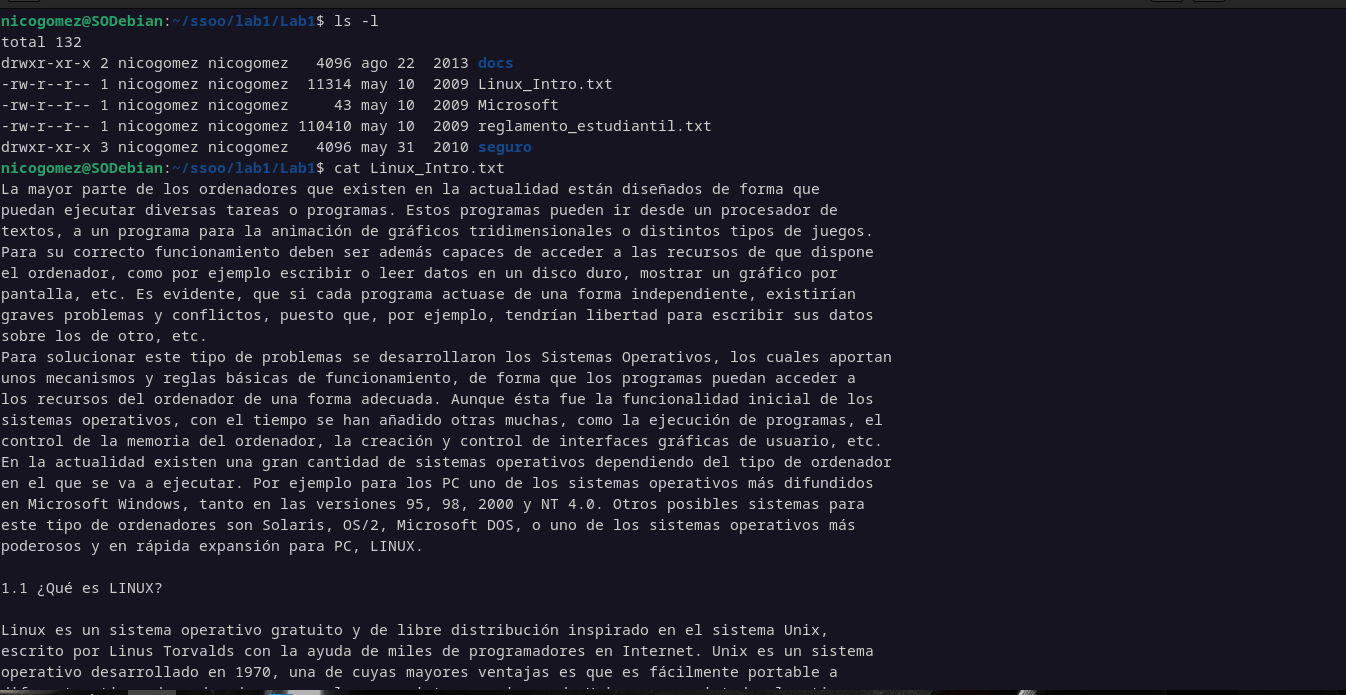
\includegraphics[width=\textwidth]{img/ejerc3a.png}
            Utilice el comando \texttt{cat Linux\ Intro.txt} para desplegar el contenido completo del archivo.
        \end{figure}
        \item Ahora despliéguelo con una herramienta que se detenga al final de cada página y espere a que usted pulse una tecla de forma que le da tiempo para leer.
        \begin{figure}[H]
            \centering
            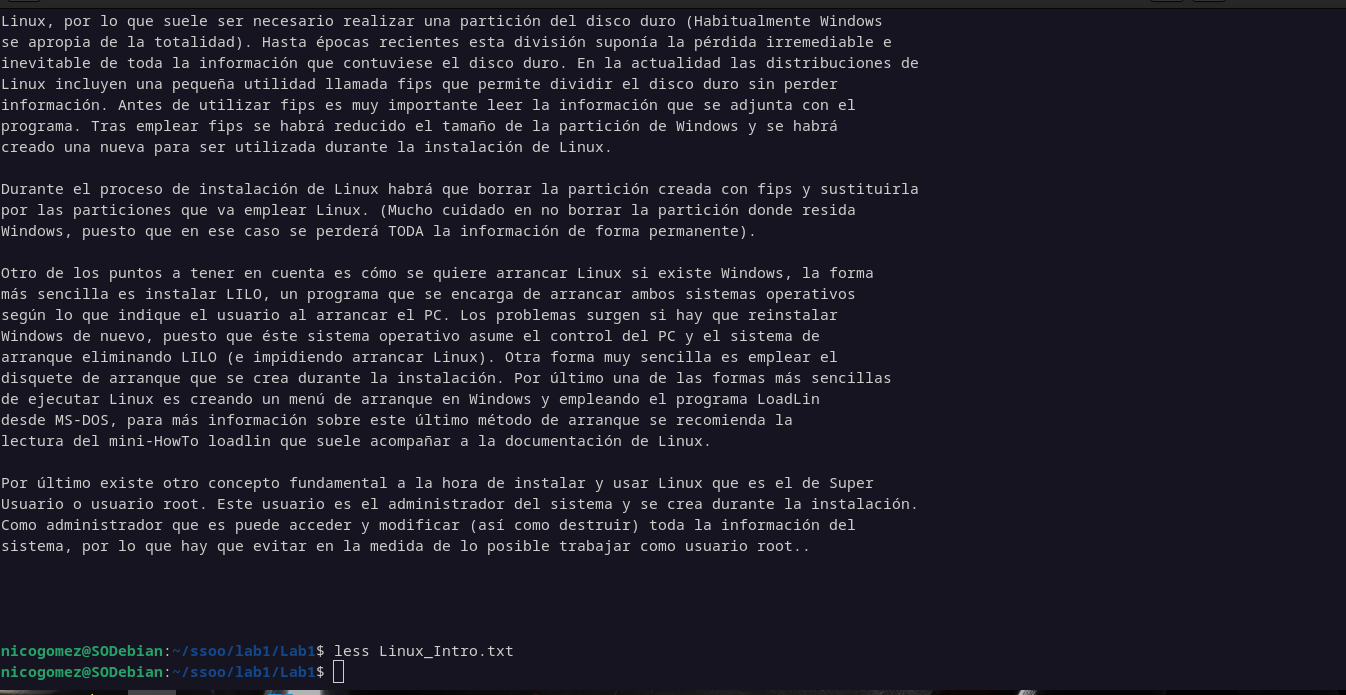
\includegraphics[width=\textwidth]{img/ejerc3b.png}
            Utilice el comando \texttt{less Linux\ Intro.txt} para desplegar el contenido completo del archivo con la herramienta \texttt{less} que permite desplazarse por el contenido con las teclas de dirección y pausar la visualización con la barra espaciadora.
        \end{figure}
        \item Busque hacia abajo/arriba en el texto las coincidencias con la palabra sistema.
        \begin{figure}[H]
            \centering
            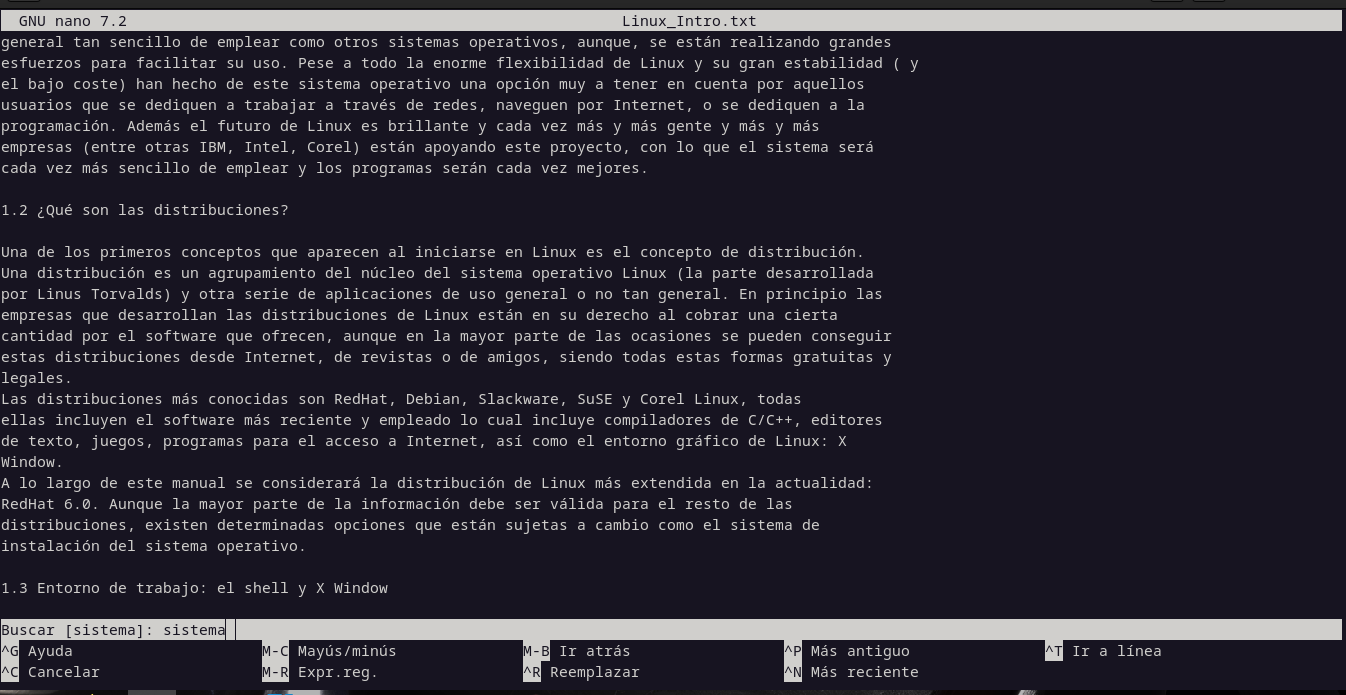
\includegraphics[width=\textwidth]{img/ejerc3c.png}
            Utilice el comando \texttt{nano Linux\ Intro.txt} para desplegar el contenido completo del archivo seguido de la combinación de teclas \texttt{Ctrl + W} para buscar la palabra \textit{sistema} y desplazarse por las coincidencias.
        \end{figure}
    \end{enumerate}
    \item Buscando contenido en uno archivo varios archivos (grep). 3pts por ítem.
    \begin{enumerate}[label=\alph*)]
        \item Busque la palabra libertad en reglamento estudiantil.txt mostrando las ocurrencias coloreadas.
        \begin{figure}[H]
            \centering
            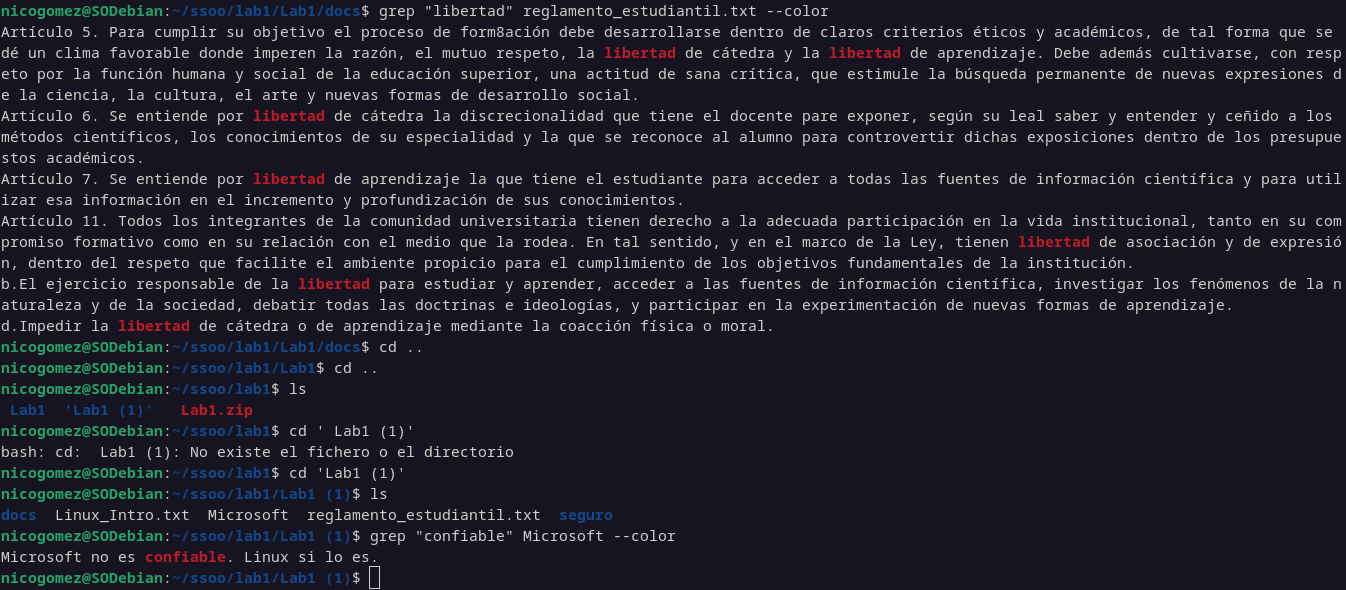
\includegraphics[width=\textwidth]{img/ejerc4a.png}
            Para este caso utilicé \texttt{grep ''libertad'' reglamento\_estudiantil.txt $--$color} 
            para buscar la palabra \textit{libertad} en el archivo \textit{reglamento\_estudiantil.txt} 
            y colorear las ocurrencias respectivamente.
        \end{figure}
        \item Busque la palabra confiable en el archivo Microsoft, mostrando las ocurrencias coloreadas.
        \begin{figure}[H]
            \centering
            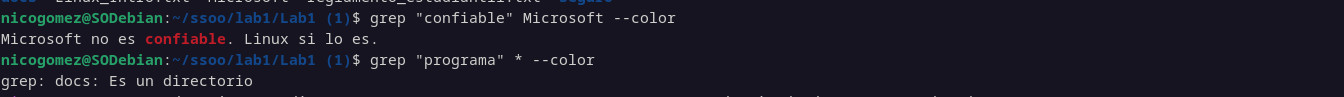
\includegraphics[width=\textwidth]{img/ejerc4b.png}
            Para este caso utilicé \texttt{grep ''confiable'' Microsoft $--$color} 
            para buscar la palabra \textit{confiable} en el archivo \textit{Microsoft} 
            y colorear las ocurrencias respectivamente.
        \end{figure}
        \item Busque la palabra programa en todos los archivos del directorio, incluido el subdirectorio docs.
        \begin{figure}[H]
            \centering
            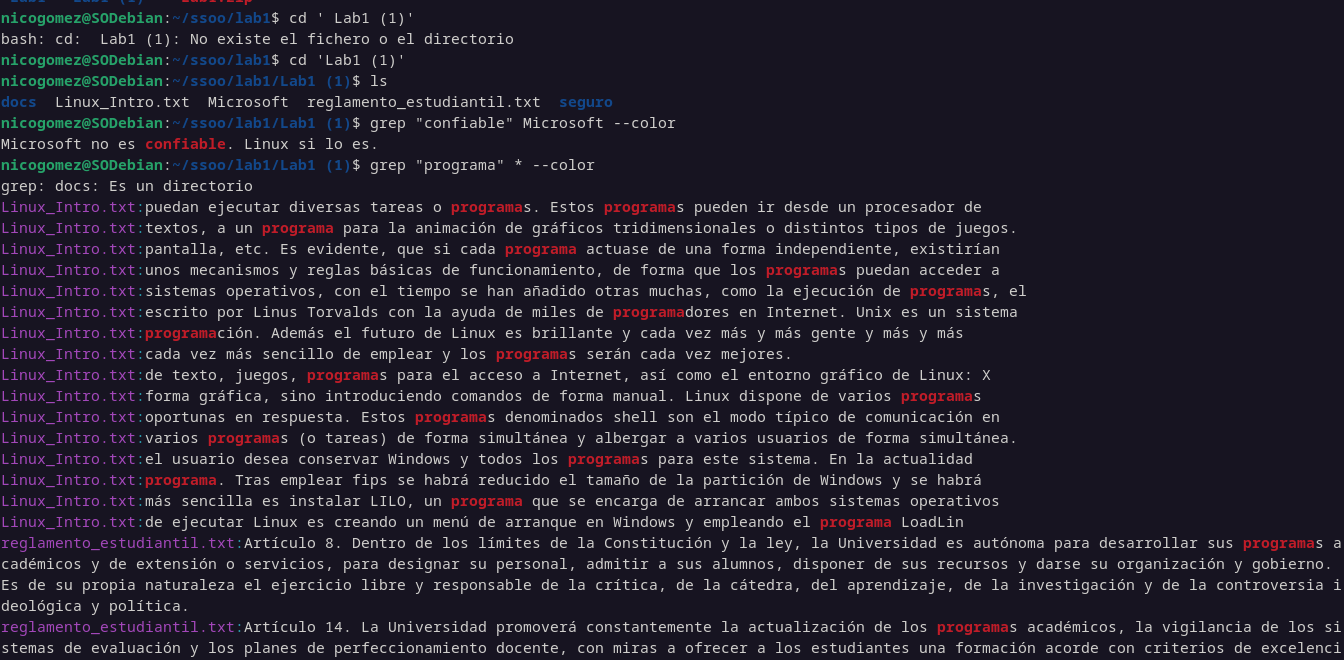
\includegraphics[width=\textwidth]{img/ejerc4c.png}
            Para este caso utilicé \texttt{grep ''programa'' * $--$color} para buscar la palabra \textit{programa} en todos los archivos y colorear las ocurrencias respectivamente.
        \end{figure}
    \end{enumerate}
    \item Haciendo cambios sobre archivos y directorios (mv, rm, mkdir). 2pts por ítem.
    \begin{enumerate}[label=\alph*)]
        \item Modifique el nombre del archivo .hidden para que no esté más oculto.
        \begin{figure}[H]
            \centering
            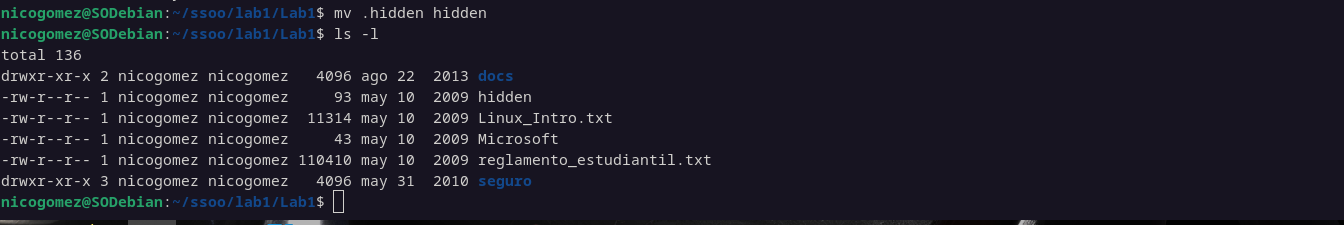
\includegraphics[width=\textwidth]{img/ejerc5a.png}
            Para este caso utilicé \texttt{mv .hidden hidden} para cambiar el nombre del archivo \textit{.hidden} a \textit{hidden}.
        \end{figure}
        \item Ingrese al directorio docs. Verifique que está en el directorio correcto.
        \begin{figure}[H]
            \centering
            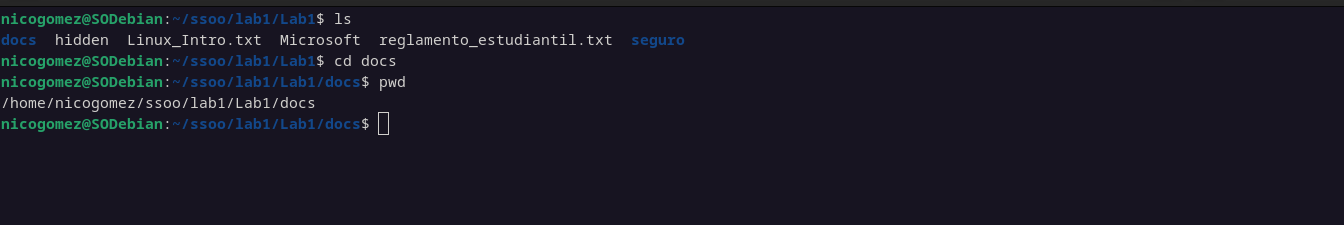
\includegraphics[width=\textwidth]{img/ejerc5b.png}
            Para este caso utilicé \texttt{cd docs/} para ingresar al directorio \textit{docs} y luego \texttt{pwd} para verificar que estaba en el directorio correcto.
        \end{figure}
        \item Mueva el archivo reglamento estudiantil.txt desde el directorio padre al directorio actual.
        \begin{figure}[H]
            \centering
            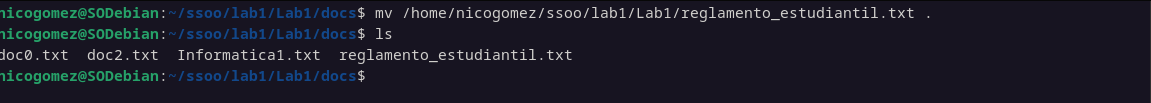
\includegraphics[width=\textwidth]{img/ejerc5c.png}
            Para este caso utilicé \texttt{mv /home/nicogomez/..../reglamento\_estudiantil.txt .} para mover el archivo \textit{reglamento\_estudiantil.txt} desde el directorio padre al directorio actual.
        \end{figure}
        \item Devuélvase al directorio padre y deshágase de una vez por todas del archivo Microsoft.
        \begin{figure}[H]
            \centering
            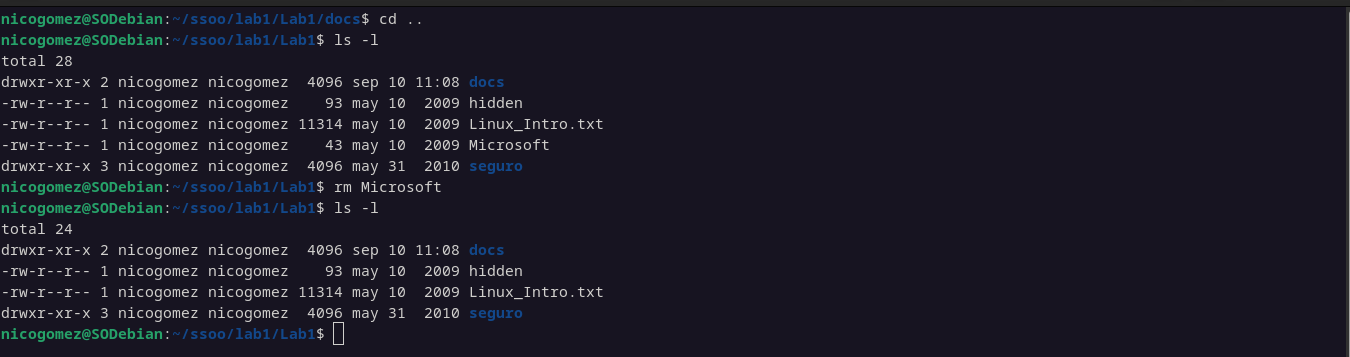
\includegraphics[width=\textwidth]{img/ejerc5d.png}
            Para este caso utilicé \texttt{cd ..} para volver al directorio padre y luego \texttt{rm Microsoft} para eliminar el archivo \textit{Microsoft}.
        \end{figure}
        \item Cree una nueva carpeta y llámela archives.
        \begin{figure}[H]
            \centering
            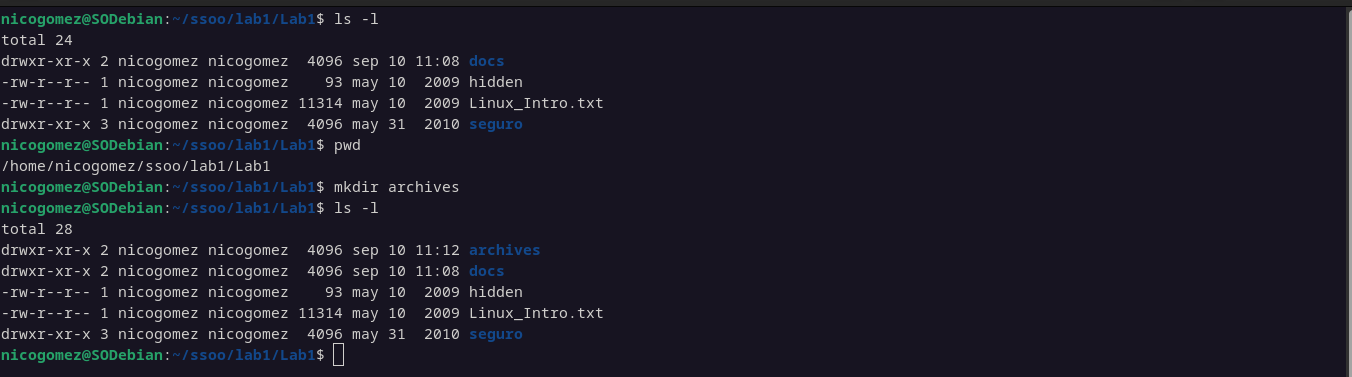
\includegraphics[width=\textwidth]{img/ejerc5e.png}
            Para este caso utilicé \texttt{mkdir archives} para crear la carpeta \textit{archives}.
        \end{figure}
        \item Copie todos los archivos de su directorio de trabajo dentro de archives, incluyendo el subdirectorio docs y todos los archivos que este contiene.
        \begin{figure}[H]
            \centering
            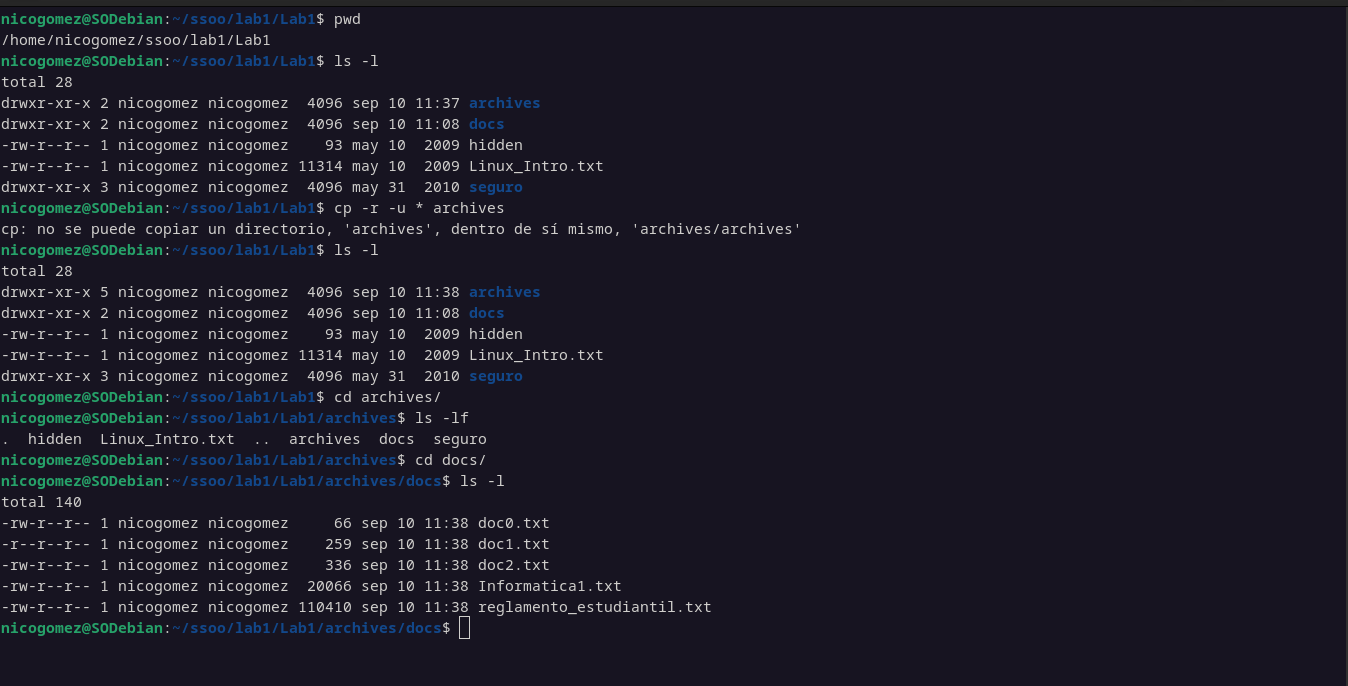
\includegraphics[width=\textwidth]{img/ejerc5f.png}
            Para este caso utilicé \texttt{cp -r -u archives} para copiar todos los archivos del directorio de trabajo dentro de \textit{archives}, incluyendo el subdirectorio \textit{docs} y todos los archivos que este contiene.
        \end{figure}
    \end{enumerate}
    \item Enlaces simbólicos (ln).  3pts por ítem.
    \begin{enumerate}[label=\alph*)]
        \item Cree enlaces simbólicos de forma que los archivos en la carpeta docs/ aparezcan también en la carpeta actual. Use una sola instrucción para tal efecto.
        \begin{figure}[H]
            \centering
            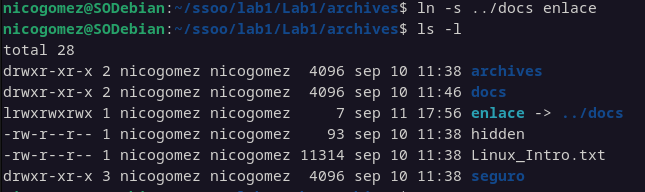
\includegraphics[width=\textwidth]{img/ejerc6a.png}
            Para este caso utilicé \texttt{ln -s ../docs enlace} para crear enlaces simbólicos de forma que los archivos en la carpeta \textit{docs/} aparezcan también en la carpeta actual.
        \end{figure}
        \item Liste los archivos en el directorio actual. ¿Cómo puede identificar los enlaces?
        \begin{center}
            Los enlaces simbólicos se identifican por el \textit{->} que aparece en la lista de archivos ademas de que mi terminal los muestra en color celeste.
        \end{center}
        \item Borre el archivo docs/doc0.txt y comente sobre el impacto en la lista de archivos del directorio actual.
        \begin{figure}[H]
            \centering
            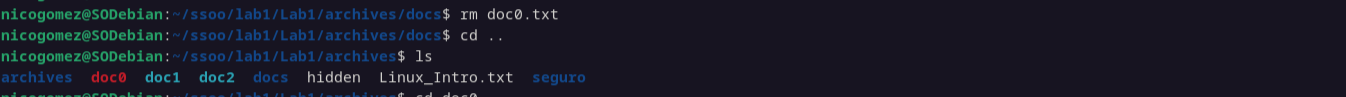
\includegraphics[width=\textwidth]{img/ejerc6c.png}
            A nivel macro en un enlace a la carpeta docs, no se ven cambios, sin embargo para enlaces directos al archivo \textit{doc0.txt} se muestra un error al intentar acceder a este.
        \end{figure}
    \end{enumerate}
    \item Derechos de acceso a archivos (chmod). 5pts por ítem.
    \begin{enumerate}[label=\alph*)]
        \item Intente borrar el archivo doc1.txt y trate de entender por qué no le está permitido hacerlo (o por qué le realiza una advertencia, si es así no lo borre todavía), para esto despliegue los derechos de acceso del archivo. Dé una explicación sobre lo sucedido.
        \begin{figure}[H]
            \centering
            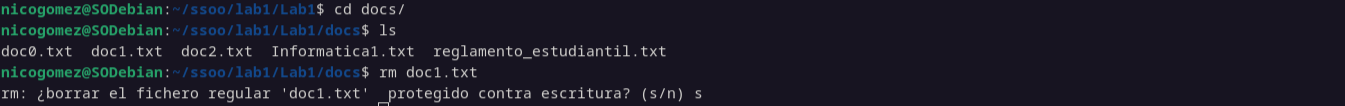
\includegraphics[width=\textwidth]{img/ejerc7a.png}
            Para este caso utilicé \texttt{rm doc1.txt} para intentar borrar el archivo \textit{doc1.txt} y me salto un mensaje de advertencia.
        \end{figure}
        Estas advertencias se dan debido a que los permisos asignados de modificación para el archivo \textit{doc1.txt} no permiten la eliminación del archivo, como se muestra en la figura anterior. Por lo que se debe modificar los permisos de acceso para poder eliminar el archivo.
        \item Modifique los derechos de acceso del archivo para que no aparezca la advertencia y elimínelo.
        \begin{figure}[H]
            \centering
            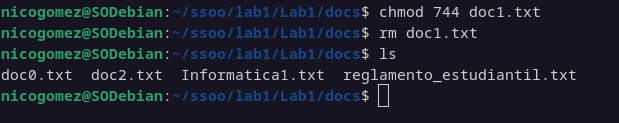
\includegraphics[width=\textwidth]{img/ejerc7b.png}
            Para este caso utilicé \texttt{chmod 744 doc1.txt} para modificar los permisos del archivo \textit{doc1.txt} y
            luego \texttt{rm doc1.txt} para eliminarlo. (el numero 744 indica los permisos que se asignan sobre el archivo).
        \end{figure}
    \end{enumerate}
    \item Redireccionamiento (history, >, cat, wc).  3pts por ítem.
    \begin{enumerate}[label=\alph*)]
        \item Regrese a la carpeta de trabajo. Un primer redireccionamiento: Use el comando history para mostrar todos los comandos que usted ya ha digitado.
        \begin{figure}[H]
            \centering
            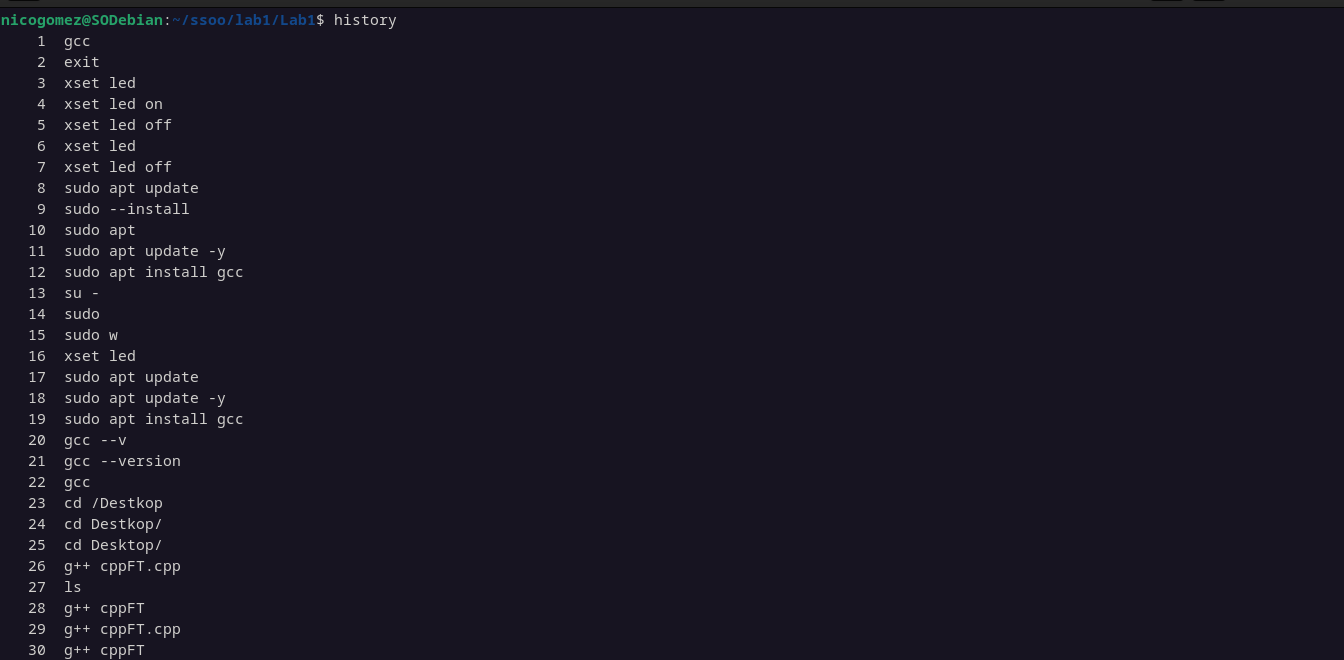
\includegraphics[width=\textwidth]{img/ejerc8a.png}
        \end{figure}
        \item Ahora guarde la salida de este comando en un nuevo archivo mihistoria.txt.
        \begin{figure}[H]
            \centering
            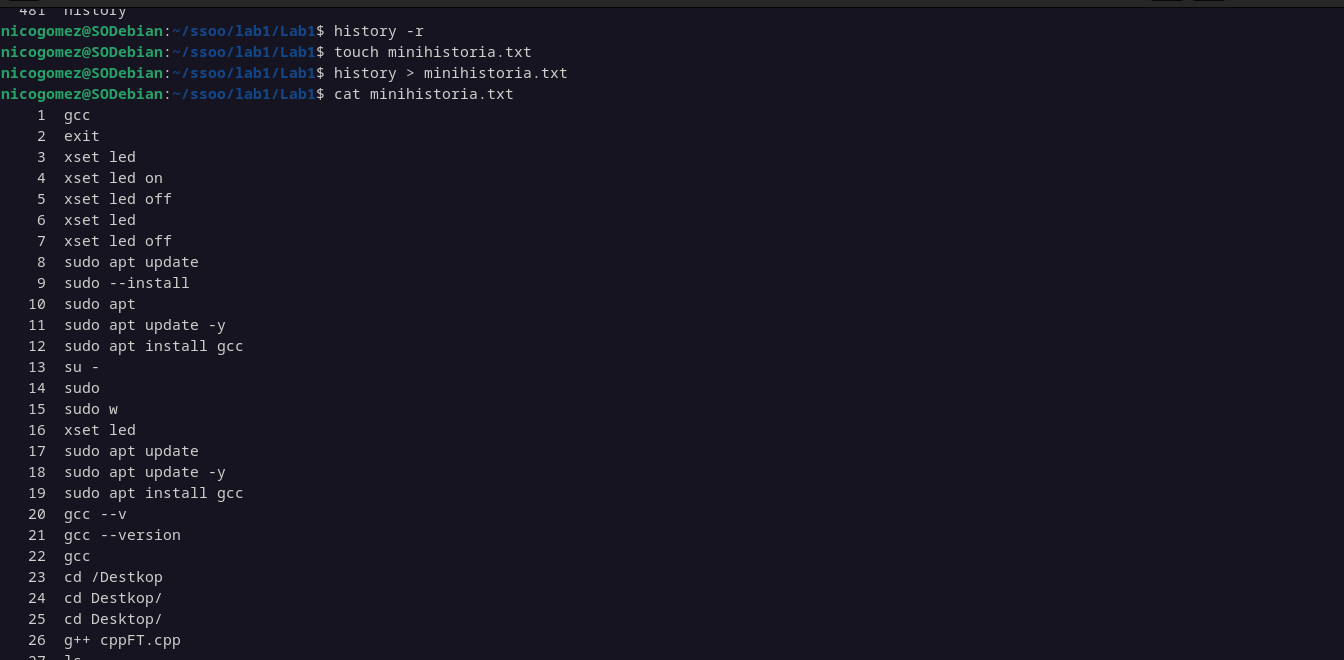
\includegraphics[width=\textwidth]{img/ejerc8b.png}
            Para este caso utilicé \texttt{history > mihistoria.txt} para guardar la salida del comando \texttt{history} en un nuevo archivo \textit{mihistoria.txt}.
        \end{figure}
        \item Concatenación de archivos: Concatene todos los archivos que están en el directorio docs/ dentro de un nuevo archivo doc3.txt sin salirse del directorio actual (Lab1). ¿Cuántas líneas, palabras y caracteres hay en el nuevo archivo?
        \begin{figure}[H]
            \centering
            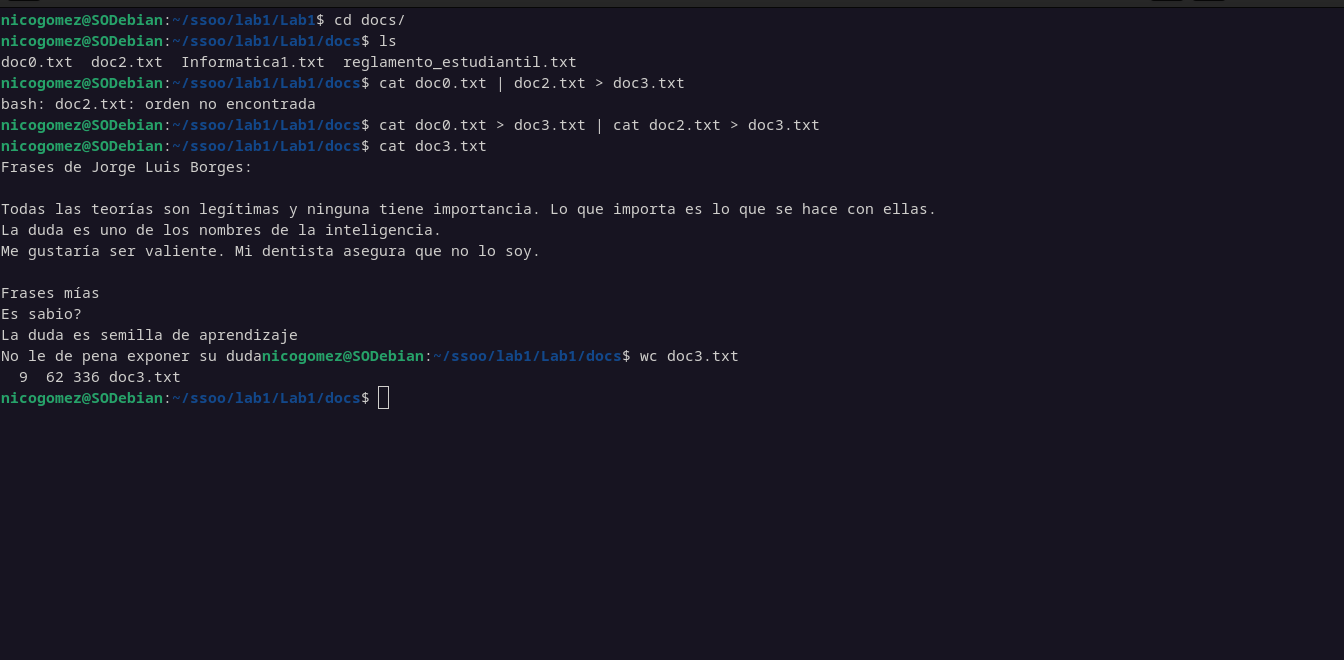
\includegraphics[width=\textwidth]{img/ejerc8c.png}
            Para este caso utilicé \texttt{cat doc0.txt > doc3.txt | cat doc2.txt > doc3.txt} para concatenar todos los archivos que están en el directorio \textit{docs/} dentro de un nuevo archivo \textit{doc3.txt} y
            luego \texttt{wc doc3.txt} para contar las líneas, palabras y caracteres del nuevo archivo. Este archivo tal como se muestra en la ultima linea de salida tiene 9 lineas, 62 palabras y 336 caracteres.
        \end{figure}
        \item Elimine el archivo doc3.txt.
        \begin{figure}[H]
            \centering
            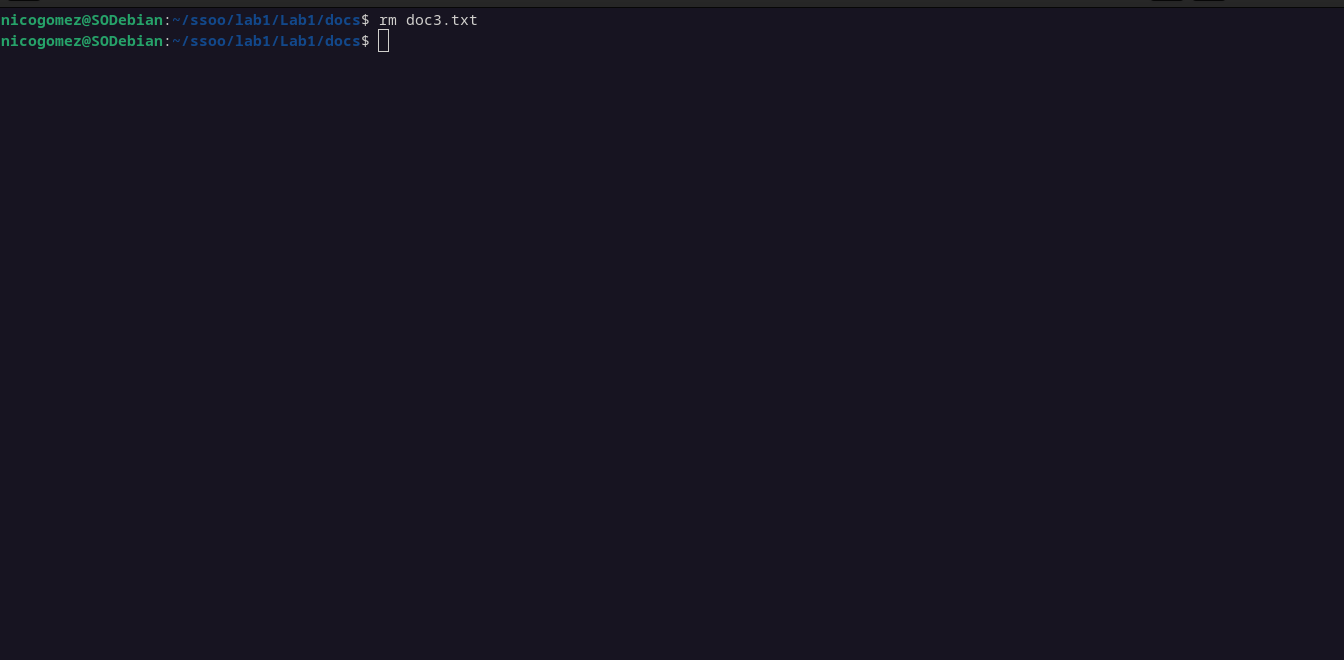
\includegraphics[width=\textwidth]{img/ejerc8d.png}
            Para este caso utilicé \texttt{rm doc3.txt} para eliminar el archivo \textit{doc3.txt}.
        \end{figure}
    \end{enumerate}
    \item Usando tuberías (|). 5pts por ítem.
    \begin{enumerate}[label=\alph*)]
        \item En una sola línea de comando despliegue todas las líneas que en los archivos del directorio docs/ contienen la palabra duda. Haga la búsqueda sin importar mayúsculas y minúsculas. Ahora obtenga el número de líneas que esto representa con una sola línea de comandos.
        \begin{figure}[H]
            \centering
            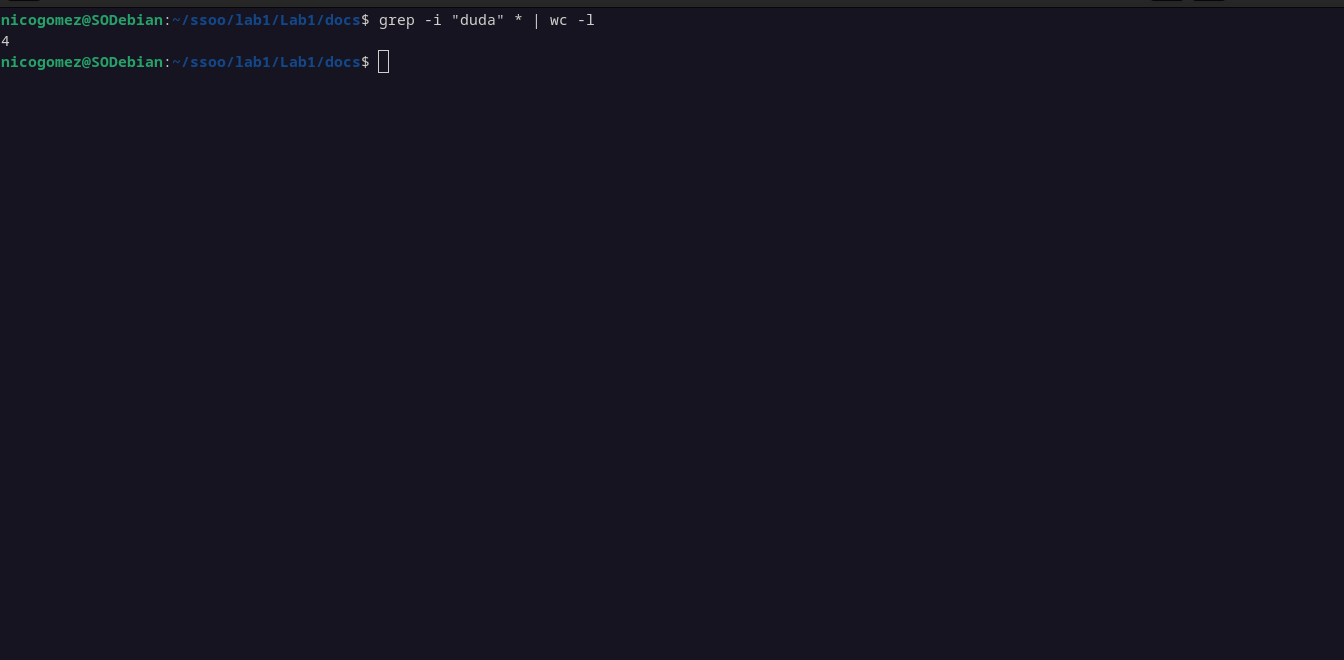
\includegraphics[width=\textwidth]{img/ejerc9a.png}
            Para este caso utilicé \texttt{grep -i ''duda'' * | wc -l} para desplegar todas las líneas que en los archivos del directorio \textit{docs/} contienen la palabra \textit{duda} sin importar mayúsculas y minúsculas (-i) y luego contar el número de líneas que esto representa con el comando \texttt{wc -l} de forma paralela.
        \end{figure}
        \item Mejore el comando anterior de modo que muestre las líneas que contienen las palabras sabio o duda. Hágalo sin importar mayúsculas y minúsculas.
        \begin{figure}[H]
            \centering
            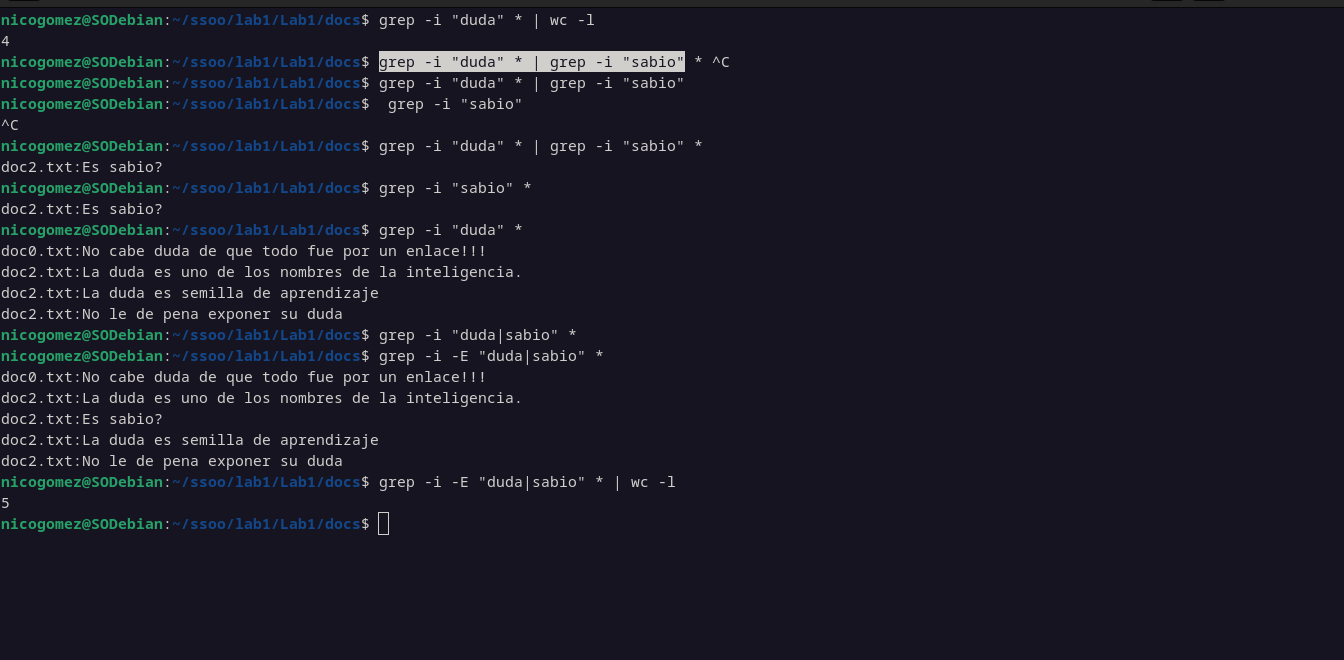
\includegraphics[width=\textwidth]{img/ejerc9b.png}
            Utilice la combinación \texttt{grep -i -E "sabio|duda" *} para mostrar las líneas que contienen las palabras \textit{sabio} o \textit{duda} sin importar mayúsculas y minúsculas y en todos los archivos del directorio.
        \end{figure}
        \item Mejore el comando anterior de modo que en con una sola línea cuente las líneas que contiene las palabras sabio o duda. Hágalo sin importar mayúsculas y minúsculas.
        \begin{figure}[H]
            \centering
            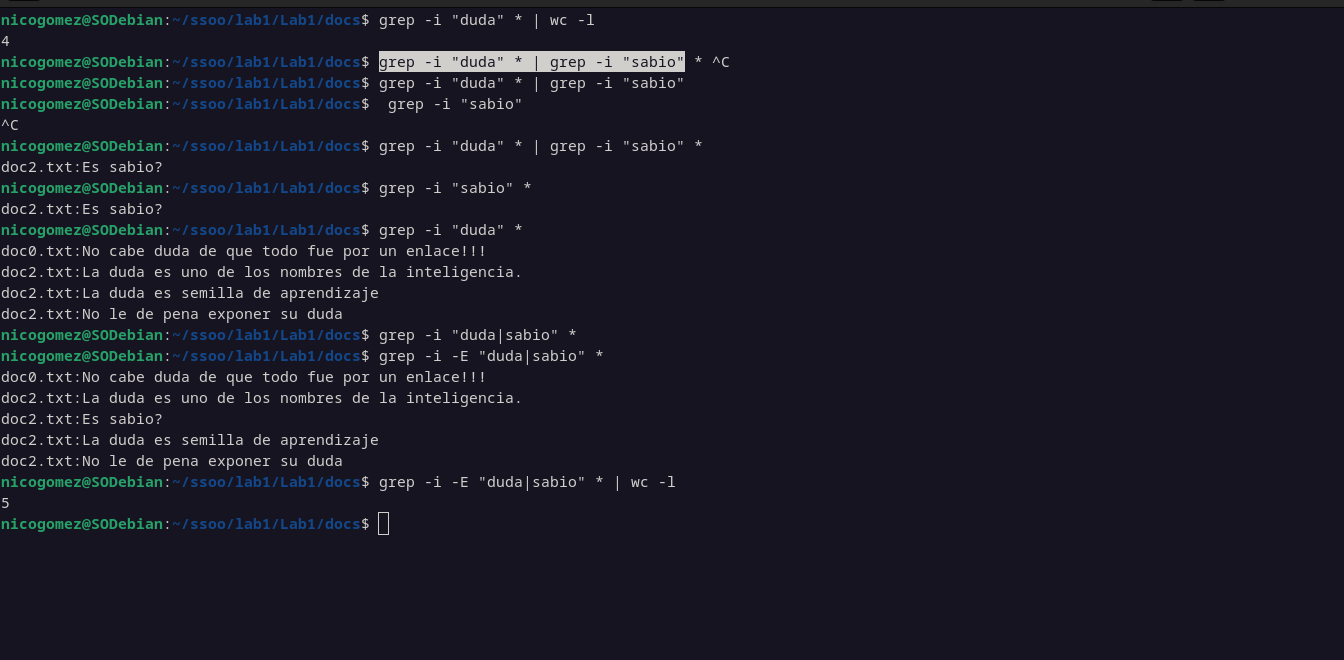
\includegraphics[width=\textwidth]{img/ejerc9b.png}
            Tal como se muestra aplique el mismo comando anterior pero con un agregado: \texttt{grep -i -E "sabio|duda" * | wc -l} para contar las líneas que contiene las palabras \textit{sabio} o \textit{duda} sin importar mayúsculas y minúsculas.    
        \end{figure}
        \item Mejore aún más el comando anterior de modo muestre las líneas que contienen las palabras sabio o duda pero que no tienen la palabra pena.
        \begin{figure}[H]
            \centering
            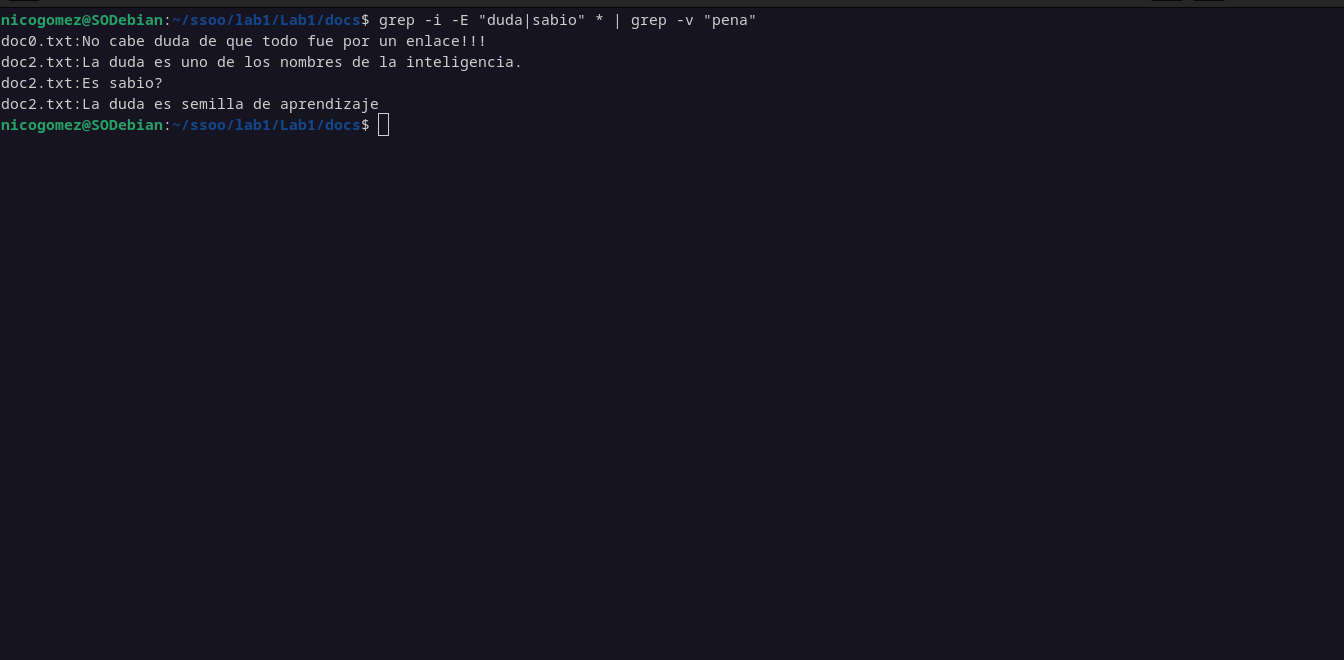
\includegraphics[width=\textwidth]{img/ejerc9d.png}
            Utilice la combinación \texttt{grep -i -E "sabio|duda" * | grep -v "pena"} para mostrar las líneas que contienen las palabras \textit{sabio} o \textit{duda} pero que no tienen la palabra \textit{pena} (\texttt{grep -v}) sin importar mayúsculas y minúsculas y en todos los archivos del directorio.
        \end{figure}
    \end{enumerate}
\end{enumerate}

\end{document}